\documentclass[12pt]{article}

% Layout.
%\usepackage[top=1in, bottom=0.75in, left=1in, right=1in, headheight=1in, headsep=6pt]{geometry}
\usepackage[margin = 1in]{geometry}

% Fonts.
\usepackage{mathptmx}
\usepackage[scaled=0.86]{helvet}
\renewcommand{\emph}[1]{\textsf{\textbf{#1}}}

% TiKZ.
\usepackage{tikz, pgfplots}
\usetikzlibrary{calc,  positioning}

% Misc packages.
\usepackage{amsmath,amssymb,latexsym}
\usepackage{graphicx}
\usepackage{array}
\usepackage{xcolor}
\usepackage{multicol}
\usepackage{fancyhdr}
\pagestyle{fancy}


% Misc.
\renewcommand{\d}{\displaystyle}
\newcommand{\ds}{\displaystyle}
\def\bc{\begin{center}}
\def\ec{\end{center}}
\def\be{\begin{enumerate}}
\def\ee{\end{enumerate}}

\newcommand{\ans}[1][1in]{\rule{#1}{.5pt}}


\lhead{Math F113X: Quiz 7}

\begin{document}

\vspace{1cm}

\noindent \textbf{Name:} \hrulefill \quad  score:\ans[1cm] \ / 10 \\


There are 10 points possible on this quiz. No aids (book, notes, etc.)
are permitted. You may use a non-programmable calculator.  {\bf Show
all work and supporting calculations for full credit. Explain how you
get your answers.}

\be
\item Consider the following directed graph.

\centering
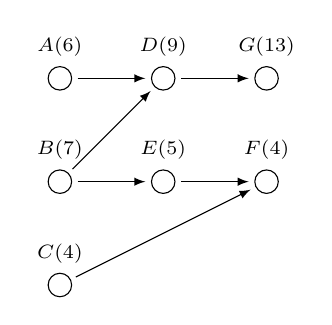
\begin{tikzpicture}[vtx/.style={draw, circle, inner sep = 3pt, font = \scriptsize}, myto/.style={-latex, shorten >=2pt, shorten <=2pt
}, node distance = 1 cm]
\node[vtx, label=above:{\scriptsize $A(6)$}, ] (A) at (0,0){};
\node[vtx, below = of A, label=above:{\scriptsize $B(7)$}] (B) {};
\node[vtx, below = of B, label=above:{\scriptsize $C(4)$}] (C) {};
\node[vtx, right = of A, label=above:{\scriptsize $D(9)$}] (D) {};
\node[vtx, right = of B, label=above :{\scriptsize $E(5)$}] (E) {};
\node[vtx, right = of E, label= above:{\scriptsize $F(4)$}] (F) {};
\node[vtx, right = of D, label=above:{\scriptsize $G(13)$}] (G) {};


\foreach \i/\j in {A/D, B/D, C/F, D/G, B/E, E/F}{\draw[myto] (\i) -- (\j);}
\end{tikzpicture}


\be
\item (1 pt) What tasks need to be completed before task D can start?

\vspace{1in}

\item (1 pt) What tasks are available to be assigned at the beginning of the project?

\vspace{1in}

\item (1 pt) What is the critical path?

\vspace{1in}


\item (1 pt) What is the critical time? \ans

\ee
\newpage

\item Suppose you have a project consisting of the seven tasks described in the following table. 


\be
\item (2 pts) Create a project digraph with vertices labeled. Draw it next to the table.

\bigskip

\begin{tabular}{| l | l |l |}\hline
label/task&time&dependence\\ \hline 
\hline
A&7&\\ \hline
B&3&\\ \hline
C&4&\\ \hline
D&3&A\\\hline
E&8&A, B\\\hline
F&2&E\\\hline

\end{tabular}

\bigskip

\item  (3 pts) Schedule the project with 2 processors using priority list
\[ A \:\quad  B\:\quad C \:\quad D \:\quad E \:\quad F \]

Make sure you write clearly so that someone else can read your schedule!

\bigskip

The finishing time is \ans and the total idle time is \ans.

\bigskip


\hspace*{-1in}	\begin{tabular}{c || c}
time &   \quad \hspace{6in} \quad \\ \hline
ready& \\ \hline
done& \\ \hline
\end{tabular}

\vspace{1.5cm}

\hspace*{-1in}
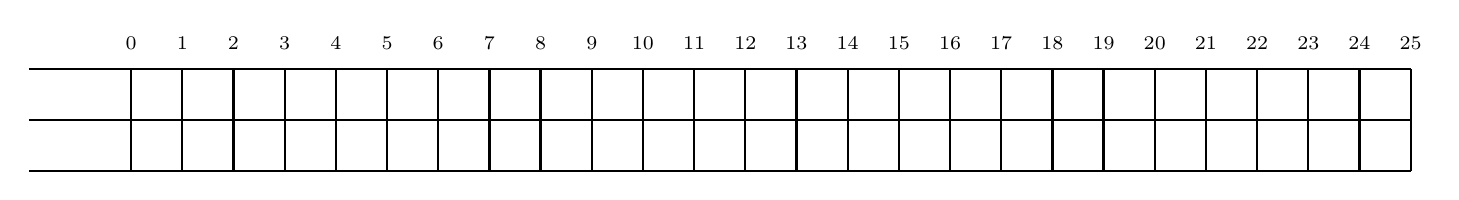
\begin{tikzpicture}[scale=.65]
\foreach \x in {0,1,...,25}{
	\node[font = \scriptsize]  at (\x,2.5){$\x$};
	\draw[thick] (\x,0) -- (\x,2);
	}
\foreach \y in {0,1,2}{\draw[thick] (-2,\y)--(25,\y);}
\end{tikzpicture}

\bigskip

\item  Create a priority list for this project based on the Decreasing-Time algorithm.

\vspace{1in}


\ee

\ee
\end{document}
%%% Local Variables:
%%% mode: LaTeX
%%% TeX-master: t
%%% End:
